\documentclass[xcolor=dvipsnames,t]{beamer} % position stuff on top of slide
% Functions, packages, etc.
%[[[
\usetheme{Frankfurt}
\usecolortheme[named=Maroon]{structure}

% Remove Navigation Symbols
\usenavigationsymbolstemplate{}

\usepackage{mathdots} % for \iddots

\usepackage{tikz}
\usetikzlibrary{matrix}
\usetikzlibrary{calc}
\tikzset{node style ge/.style={circle}}

\usepackage{amsmath}
\usepackage{amsfonts}
\usepackage{amssymb}
\usepackage{amsthm}
\usepackage{array}

\usepackage{tikz,gnuplot-lua-tikz}
%\usetikzlibrary{external} % speed up TikZ compilation by caching figures; use lualatex over pdflatex (dynamic memory alloc)
%%XXX need to add -enable-write18 to initial lualatex call in Makefile
%\tikzexternalize[prefix=tikz_cache/]
%\tikzset{external/system call={lualatex
%      \tikzexternalcheckshellescape -halt-on-error -interaction=batchmode
%-jobname "\image" "\texsource"}}%

\usepackage{graphicx}
%\usepackage{subfig}
\usepackage[labelfont=bf]{caption}
%\usepackage[labelfont=bf]{subcaption}
%\usepackage[top=1in, bottom=1in, left=1in, right=1in]{geometry}
%\pagenumbering{arabic}
\usepackage{hyperref}
%\numberwithin{equation}{section}
%\usepackage{soul} % for \ul - a ``better'' underlining command

%\usepackage{colortbl} % for coloring \multicolumn (tabular in general, I think)
% For \rowcolor
%\definecolor{table_header}{gray}{0.5}
%\definecolor{table_data}{gray}{0.85}

\usepackage{algorithm}
\usepackage{algpseudocode,algorithmicx}

%% Inserting code and syntax highlighting
%% [[[
%\usepackage{listings} % like verbatim, but allows for syntax highlighting and more
%\usepackage{color} % colors
%\usepackage[usenames,dvipsnames]{xcolor}% More colors
%\usepackage{caption} % captions
%\DeclareCaptionFont{white}{\color{white}}
%\DeclareCaptionFormat{listing}{\colorbox{gray}{\parbox{\textwidth}{#1#2#3}}}
%\captionsetup[lstlisting]{format=listing,labelfont=white,textfont=white}
%\usepackage{framed} % put a frame around things
%
%% define some custom colors
%\definecolor{dkgreen}{rgb}{0,0.6,0}
%\definecolor{lgreen}{rgb}{0.25,1,0}
%\definecolor{purple}{rgb}{0.35,0.02,0.48}
%
%% Some changes to MATLAB/GNU Octave language in listings
%\lstset{frame=tbrl,
%    language=Matlab,
%    aboveskip=3mm,
%    belowskip=3mm,
%    belowcaptionskip=3mm,
%    showstringspaces=false,
%    columns=flexible,
%    basicstyle={\small\ttfamily\color{black}},
%    numbers=left,
%    numberstyle=\tiny\color{purple},
%    keywordstyle=\color{dkgreen},
%    commentstyle=\color{red},
%    stringstyle=\color{purple},
%    breaklines=true,
%    breakatwhitespace=true,
%    tabsize=4,
%    rulecolor=\color{black},
%    morekeywords={string,fstream}
%}
%% ]]]


%My Functions
\newcommand{\diff}[2]{\dfrac{d #1}{d #2}}
\newcommand{\diffn}[3]{\dfrac{d^{#3} #1}{d {#2}^{#3}}}
\newcommand{\pdiff}[2]{\dfrac{\partial #1}{\partial #2}}
\newcommand{\pdiffn}[3]{\dfrac{\partial^{#3} #1}{\partial {#2}^{#3}}}
\newcommand{\problemline}{\rule{\textwidth}{0.25mm}}
%\newcommand{\problem}[1]{\problemline\\#1\\\problemline\vspace{10pt}}
\newcommand{\reals}{\mathbb{R}}
\newcommand{\qline}[2]{\qbezier(#1)(#1)(#2)}
\newcommand{\abox}[1]{\begin{center}\fbox{#1}\end{center}}
\newcommand{\lie}{\mathcal{L}}
%\newcommand{\defeq}{\stackrel{\operatorname{def}}{=}}

% AMS theorem stuff
%% [[[
%\newtheoremstyle{mystuff}{}{}{\itshape}{}{\bfseries}{:}{.5em}{}
%\theoremstyle{mystuff}
%\newtheorem{definition}{Definition}[section]
%\newtheorem*{definition*}{Definition}
%\newtheorem{theorem}{Theorem}[section]
%\newtheorem*{theorem*}{Theorem}
%\newtheorem{lemma}{Lemma}[section]
%\newtheorem*{lemma*}{Lemma}
%\newtheorem{proposition}{Proposition}[section]
%\newtheorem*{proposition*}{Proposition}
%\newtheorem*{corollary*}{Corollary}
%\newtheorem*{remark}{Remark}
%
%\newtheoremstyle{myexample}{}{}{}{}{\bfseries}{:}{.5em}{}
%\theoremstyle{myexample}
%\newtheorem*{example*}{Example}
%
%% Stolen from http://tex.stackexchange.com/questions/8089/changing-style-of-proof
%\makeatletter \renewenvironment{proof}[1][\proofname] {\par\pushQED{\qed}\itshape\topsep6\p@\@plus6\p@\relax\trivlist\item[\hskip\labelsep\bfseries#1\@addpunct{:}]\ignorespaces}{\popQED\endtrivlist\@endpefalse} \makeatother
%
%% Stolen from http://tex.stackexchange.com/questions/12913/customizing-theorem-name
%\newtheoremstyle{named}{}{}{\itshape}{}{\bfseries}{:}{.5em}{\thmnote{#3's }#1}
%\theoremstyle{named}
%\newtheorem*{namedtheorem}{Theorem}
%% ]]]

%]]]


% Output Control Variables
\def\true{1}
\def\false{0}
\def\figures{1}
\def\tables{1}

\renewcommand{\UrlFont}{\scriptsize}
\newcommand{\defeq}{\mathrel{\mathop:}=}
\DeclareMathOperator*{\argmin}{arg\,min}

% http://tex.stackexchange.com/questions/43065/matrices-too-big-to-fit-the-width-of-a-page
\newcommand\scalemath[2]{\scalebox{#1}{\mbox{\ensuremath{\displaystyle #2}}}}

\title{Application of Adjoint Operators in Gradient Computations}
\date{5 March, 2016}
\author{James Folberth\\Advisor: Stephen Becker}
\institute{University of Colorado at Boulder}

\begin{document}

\begin{frame}
\maketitle
\end{frame}

\begin{frame}{Outline}
   \begin{enumerate}
      \item A generic optimiztion problem
      \item Example 1: Image Deblurring
      \item Example 2: Blind Channel Estimation
   \end{enumerate}

   \begin{center}
   \begin{columns}[b]
      \begin{column}{0.45\textwidth}
         \begin{center}
         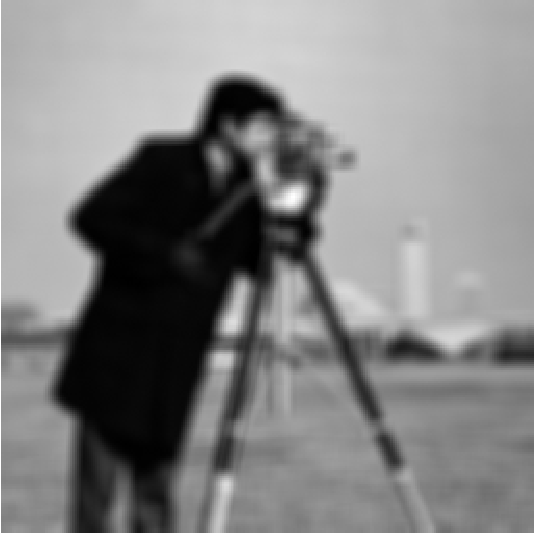
\includegraphics[width=0.8\textwidth]{../ieee_spm/figures/cameraman_observed_trim.pdf}
         \end{center}
      \end{column}
      
      \begin{column}{0.45\textwidth}
         \begin{center}
         \includegraphics[width=0.8\textwidth]{../ieee_spm/figures/{cameraman_rec_200_bior4.4_sym_trim}.pdf}
         \end{center}
      \end{column}
   \end{columns}
   \end{center}


\end{frame}

\section{Generic Problem}
% [[[
\begin{frame}{A Generic Problem}
   Consider

   \[ \min_x \dfrac{1}{2}\|\mathcal{A}x-b\|_2^2 + \lambda \|x\|_1. \] 

   \begin{itemize}
      \item $\mathcal{A}$ is a linear operator on problem variable $x$.
      \item $b$ is measured data (e.g. blurry image).
      \item Include $\lambda \|x\|_1$, to induce sparsity in $x$ (hopefully).
   \end{itemize}

   Define 

   \[ f(x) = \dfrac{1}{2}\|\mathcal{A}x-b\|_2^2, \quad g(x) = \lambda \|x\|_1. \] 

   \noindent $f(x)$ is convex, differentiable, $g(x)$ is convex, non-differentiable.
   
   \[ \nabla f(x) = \mathcal{A}^\ast\left(\mathcal{A}x-b\right). \] 

\end{frame}

\begin{frame}{Proximal Gradient Method}
   \[ \min_x \dfrac{1}{2}\|\mathcal{A}x-b\|_2^2 + \lambda \|x\|_1. \] 

   \[ \nabla f(x) = \mathcal{A}^\ast\left(\mathcal{A}x-b\right), \quad x^{+} = \operatorname{prox}_{t g}\left(x - t\nabla f(x)\right). \] 

   \noindent Need to efficiently compute
   \begin{itemize}
      \item $\operatorname{prox}_{tg}(x)$ with $g(x) = \lambda \|x\|_1$.  ``Shrinkage'' is fast.
      \item $\mathcal{A}$.  Usually have fast forward and inverse transform (e.g. FFT, discrete wavelet transform).
      \item $\mathcal{A}^\ast$.  Sometimes not so easy...  Let's look at a couple examples.
   \end{itemize}
\end{frame}

% ]]]


\section{Image Deblurring}
% [[[
\begin{frame}{Image Deblurring Problem}
   Observation: natural images tend to have sparse wavelet coefficients.\\
   
   \begin{itemize}
      \item $b$ - observed blurred image, with known blurring operator $\mathcal{R}$\\ (e.g. Gaussian PSF applied efficiently in Fourier domain)
      \item $\mathcal{W}$ - multi-level wavelet synthesis operator
      \item $x$ - wavelet coefficients
   \end{itemize}

   Natural problem formulation is

   \[ \min_x \dfrac{1}{2}\left\|\mathcal{RW}x-b\right\|_2^2 + \lambda \|x\|_1. \]

   \[ \nabla f(x) = \mathcal{W}^\ast\mathcal{R}^\ast\left(\mathcal{RW}x-b\right). \] 

\end{frame}

\begin{frame}{Image Deblurring Problem}
   \begin{center}
   \begin{columns}[t]
      \begin{column}{0.45\textwidth}
         Observed image:
         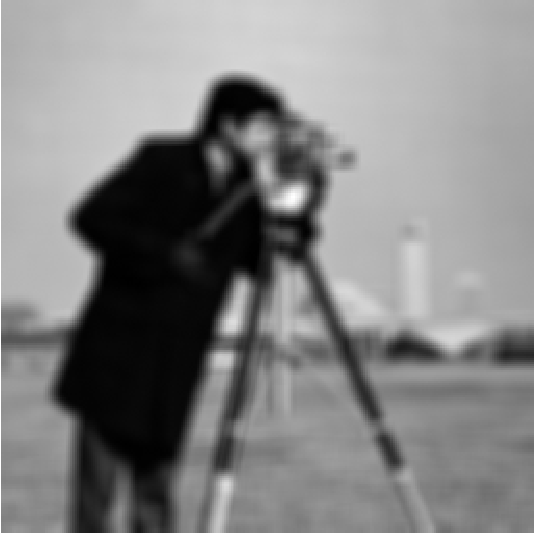
\includegraphics[width=\textwidth]{../ieee_spm/figures/cameraman_observed_trim.pdf}
      \end{column}
      
      \begin{column}{0.45\textwidth}
         Recovered image:
         \includegraphics[width=\textwidth]{../ieee_spm/figures/{cameraman_rec_200_bior4.4_sym_trim}.pdf}
      \end{column}
   \end{columns}
   \end{center}
\end{frame}

\begin{frame}{Adjoint of Wavelet Operator}
   \[ \nabla f(x) = \mathcal{W}^\ast\mathcal{R}^\ast\left(\mathcal{RW}x-b\right). \] 
   
   \begin{itemize}
      \item $\mathcal{W}$ is wavelet synthesis (reconstruction).  Standard routine in libraries.
      % actually DCT is used for symmetric/reflexive BCs
      \item $\mathcal{R}$ and $\mathcal{R}^\ast$ for blurring PSF can be applied rapidly in Fourier domain (FFT).
      \item What about $\mathcal{W}^\ast$?  Not a standard operation like $\mathcal{W}$ and $\mathcal{W}^\dagger$.
   \end{itemize}

   If $\mathcal{W}$ is orthogonal, $\mathcal{W}^\ast = \mathcal{W}^\dagger$.\\
   If $\mathcal{W}$ is biorthogonal, $\mathcal{W}^\ast \approx \mathcal{W}^\dagger$.\\
   So, one option is

   \[ \nabla f(x) \approx \mathcal{W}^\dagger\mathcal{R}^\ast\left(\mathcal{RW}x-b\right). \]
   
   % And many people use this approach.  It actually works pretty well.  But how much error does W^* = W^+ indtroduct?
\end{frame}

\begin{frame}{Adjoint of Wavelet Operator}
   We could use $\mathcal{W}^\ast \approx \mathcal{W}^\dagger$, but it turns out we can find the adjoint exactly!\\
   
   \begin{itemize}
      \item Related to $\mathcal{W}$ are frame vectors $\phi_n$ (the wavelet basis vectors), which define a frame operator $\Phi=\mathcal{W}^\dagger$:

         \[ \Phi f[n] = \langle f, \phi_n\rangle. \] 
      \item We can define the dual frame vectors $\tilde{\phi}_n=\left(\Phi^\ast\Phi\right)^{-1}\phi_n$.
      \item Define the dual frame operator via

         \[ \tilde{\Phi}f[n] = \langle f, \tilde{\phi}_n\rangle. \] 

      \item Digging around in frame theory a bit, we find

         \[ \Phi^\ast = \tilde{\Phi}^\dagger \implies {\color{blue}\mathcal{W}^\ast = \tilde{\mathcal{W}}^\dagger}\] 
   \end{itemize}

\end{frame}

\begin{frame}{Adjoint of Wavelet Operator}
   So we have $\mathcal{W}^\ast = \tilde{\mathcal{W}}^\dagger$: the adjoint of wavelet synthesis is dual wavelet analysis.\\

   But we must also handle boundary conditions.\\

   This is usually done by extending the signal via $\mathcal{E}$ to satisfy the BCs.\\

   The relation $\mathcal{W}^\ast = \tilde{\mathcal{W}}^\dagger$ holds for $\mathcal{E}$ being zero-padding, since $\mathcal{E}_\text{zpd}^\ast = \mathcal{E}_\text{zpd}^\dagger$.  Let $\mathcal{W}_\text{zpd}$ be wavelet synthesis with zero BCs.\\

   In general, we have

   \[ \mathcal{W}^\dagger = \mathcal{W}_\text{zpd}^\dagger\mathcal{E} \implies \mathcal{W}=\mathcal{E}^\dagger\mathcal{W}_\text{zpd} \implies \mathcal{W}^\ast = \mathcal{W}_\text{zpd}^\ast\left(\mathcal{E}^\dagger\right)^\ast \]

   and

   \[ {\color{blue} \mathcal{W}^\ast = \tilde{\mathcal{W}}_\text{zpd}^\dagger \left(\mathcal{E}^\dagger\right)^\ast}. \] 


\end{frame}

\begin{frame}{Adjoint of Pseudoinverse Extension}
   Due to factorization $\mathcal{W}^\ast = \tilde{\mathcal{W}}_\text{zpd}^\dagger(\mathcal{E}^\dagger)^\ast$, we just need to implement $(\mathcal{E}^\dagger)^\ast$!  $\tilde{\mathcal{W}}_\text{zpd}^\dagger$ is a standard and fast operation.\\[.5em]

   Consider a signal $y[n]$, $n=0,...,N-1$.  Let $L_p$ be the length of wavelet analysis filters.\\[.5em]

   Zero padding:
   \[ \underbrace{0, ..., 0}_{L_p-1}, y[0], ..., y[N-1], \underbrace{0, ..., 0}_{L_p-1}. \]

   Half-point symmetric:
   \[ \underbrace{y[L_p-1], ..., y[0]}_\text{Left extension}, y[0], ..., y[N-1], \underbrace{y[N-1], ..., y[N+L_p-2]}_\text{Right extension}. \] 

\end{frame}

\begin{frame}{Zero padding}
   Zero padding as a linear operator:

   \begin{columns}
      \begin{column}{0.7\textwidth}
\[ \mathcal{E}_\text{zpd} = \begin{bmatrix} 0_{(L_p-1)\times N}\\ I_{N\times N}\\ 0_{(L_p-1)\times N}\end{bmatrix} = \begin{bmatrix} 0 & 0 & \cdots & 0 & 0\\ \vdots & \vdots &\ddots & \vdots & \vdots\\ 0 & 0 & \cdots & 0 & 0\\[0.5em] 1 & 0 & \cdots & 0 & 0\\ 0 & 1 & \cdots & 0 & 0\\ \vdots & \vdots & \ddots & \vdots & \vdots\\ 0 & 0 & \cdots & 1 & 0\\ 0 & 0 & \cdots & 0 & 1\\[0.5em] 0 & 0 & \cdots & 0 & 0\\ \vdots & \vdots & \ddots & \vdots & \vdots\\ 0 & 0 & \cdots & 0 & 0\end{bmatrix}. \] 
      \end{column}

      \begin{column}{0.3\textwidth}
         In this case

         \[ \left(\mathcal{E}_\text{zpd}^\dagger\right)^\ast = \mathcal{E}_\text{zpd}. \] 

         \noindent This is what allows us the factorization

         \[ \mathcal{W}^\ast = \tilde{\mathcal{W}}_\text{zpd}^\dagger \left(\mathcal{E}^\dagger\right)^\ast. \] 


      \end{column}
   \end{columns}
\end{frame}

\begin{frame}{Half-point symmetric}
   Half-point symmetric extension as a linear operator:

\[ \scalemath{0.75}{\mathcal{E}_\text{sym} = \begin{bmatrix} & & \iddots & & &\\ & 1 &&&&\\ 1&&&&&\\1&&&&\\&1&&&&\\&&\ddots&&&\\&&&1&\\&&&&1\\&&&&1\\&&&1&\\&&\iddots&&\end{bmatrix}, \quad \left(\mathcal{E}_\text{sym}^\dagger\right)^\ast = \scalemath{0.75}{\begin{bmatrix} & \iddots \\ 1/2&&&&&\\1/2&&&&\\&\ddots&&&&&&\\&&1/2&\\&&&1\\&&&&\ddots\\&&&&&1\\&&&&&&1/2\\&&&&&&&\ddots\\&&&&&&&&1/2\\&&&&&&&&1/2\\&&&&&&&\iddots\\\end{bmatrix}}}. \]

\end{frame}

\begin{frame}{Image Deblurring Problem}
   \begin{itemize}
      \item $\mathcal{W}^\ast = \tilde{\mathcal{W}}_\text{zpd}^\dagger(\mathcal{E}^\dagger)^\ast$.
      \item $\tilde{\mathcal{W}}^\dagger$ is part of wavelet libraries and is fast.
      \item $(\mathcal{E}^\dagger)^\ast$ is closed-form (once you find it) and fast.
      \item So we can apply $\mathcal{W}^\ast$ efficiently \emph{and correctly} in

         \[ \nabla f(x) = \mathcal{W}^\ast\mathcal{R}^\ast\left(\mathcal{RW}x-b\right). \] 
   \end{itemize}
\end{frame}

\begin{frame}{Image Deblurring Problem}
   $200$ iterations of FISTA, $\mathcal{W}^\dagger$ is a 3-stage CDF 9/7 wavelet transform, ${\lambda = 2\times 10^{-5}}$
   \begin{center}
   \begin{columns}[t]
      \begin{column}{0.45\textwidth}
         Using $\mathcal{W}^\ast \approx \mathcal{W}^\dagger$:
         \includegraphics[width=\textwidth]{../ieee_spm/figures/{cameraman_rec_200_bior4.4_sym_badjoint_trim}.pdf}

         \[ \scalemath{0.75}{\dfrac{\|\mathcal{W}x-y\|_2}{\|y\|_2} = 7.25\times 10^{-2}} \] 
      \end{column}
      
      \begin{column}{0.45\textwidth}
         Using $\mathcal{W}^\ast = \tilde{\mathcal{W}}_\text{zpd}^\dagger(\mathcal{E}^\dagger)^\ast$:
         \includegraphics[width=\textwidth]{../ieee_spm/figures/{cameraman_rec_200_bior4.4_sym_trim}.pdf}
         \[ \scalemath{0.75}{\dfrac{\|\mathcal{W}x-y\|_2}{\|y\|_2} = 7.24\times 10^{-2}} \] 
      \end{column}
   \end{columns}
   \end{center}

\end{frame}

% ]]]


\section{Blind Channel Estimation}
% [[[
\begin{frame}{BCE Problem}
   %TODO could change output signals to y_i and y?  Doesn't match BCE literature, but works better with above
   Unknown source $s$ sends signal over unknown channels with impulse responses $h_i$.  We observe channel outputs

   \[ x_i[n] = \{h_i\ast s\}[n]. \] 
   
   \noindent Can we recover source and channel IRs?\\

   Let's restrict ourselves to $h_i$ and $s$ real-valued.

   Notice that for any $\alpha\neq 0$, 

   \[ x_i[n] = \{h_i\ast s\}[n] = \{\alpha h_i \ast \dfrac{1}{\alpha} s\}[n]. \] 

   \noindent So we can maybe recover $h_i$ and $s$ up to a factor.

\end{frame}

\begin{frame}{BCE Problem}
   For simplicity of notation, consider a single channel $h$ with output $x$.  Let $h$ be of length $K$ and $s$ be of length $N$; $x$ will be of length $K+N-1$.\\[0.5em]

   One can write the convolution as linear operator on the $K\times N$ matrix $hs^T$:

   \[ x = h\ast s = \mathcal{A}(hs^T). \] 

   \noindent Assuming $h$ and $s$ should be sparse in time, a natural problem formulation is
      
   \[ \min_{h,s} \dfrac{1}{2}\|\mathcal{A}(hs^T)-x\|_2^2 + \lambda_h\|h\|_1 + \lambda_s\|s\|_1. \] 

   \noindent This is non-convex.  Can use other regularization terms (e.g. $\|h\|_\text{TV}$).
\end{frame}

\begin{frame}{Adjoint of $\mathcal{A}$}
   Define $f(h,s) = 1/2\|\mathcal{A}(hs^T)-x\|_2^2$.\\[.5em]
   
   The required gradients are
   \begin{align*}
      \nabla_h f(h,s) &= \left[\mathcal{A}^\ast(\mathcal{A}(hs^T)-x)\right]s\\
      \nabla_s f(h,s) &= \left[\mathcal{A}^\ast(\mathcal{A}(hs^T)-x)\right]^Th.
   \end{align*}

   Note that $\mathcal{A}$ takes a matrix and returns a vector.  So $\mathcal{A}^\ast$ must take a vector and return a matrix (of appropriate size).\\

\end{frame}

\begin{frame}{Adjoint of $\mathcal{A}$}
   We know the action of $\mathcal{A}(hs^T)$:
      
   \[ x[n] =  \sum_{k=k_1(n)}^{k_2(n)} h[k]s[n-k], \] 

   where $k_1(n) = \max\{0,n+1-N\}$ and $k_2(n) = \min\{K-1,n\}$.

\end{frame}

\begin{frame}{Adjoint of $\mathcal{A}$}
   We know the action of $\mathcal{A}(hs^T)$:

   \begin{center}
   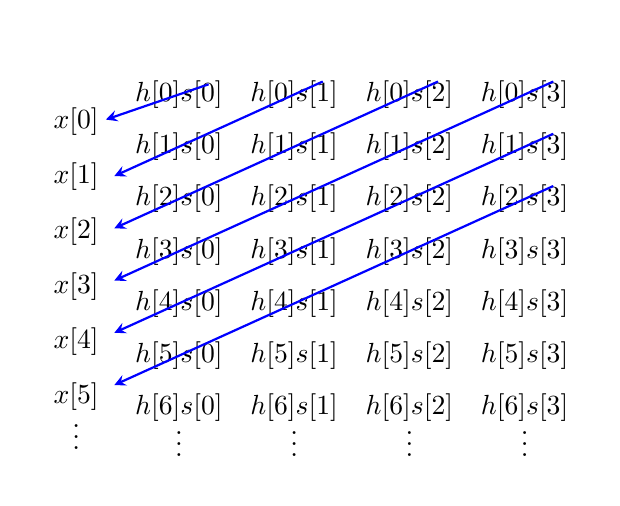
\begin{tikzpicture}[baseline=(hs.center), ampersand replacement=\&]
      % [[[
      % based on figure from Romberg et al. "Multichannel blind deconvolution..."
      % and examples from http://www.texample.net/tikz/examples/mnemonic-rule-for-matrix-determinant/
      % http://tex.stackexchange.com/questions/83046/position-two-stacked-tikz-matrices
      % http://www.texample.net/tikz/examples/energy-level-diagram/
      \matrix (hs) [matrix of math nodes, nodes = {node style ge},, column sep=0mm, row sep=-8mm]
      {h[0]s[0] \& h[0]s[1] \& h[0]s[2] \& h[0]s[3] \\
       h[1]s[0] \& h[1]s[1] \& h[1]s[2] \& h[1]s[3] \\
       h[2]s[0] \& h[2]s[1] \& h[2]s[2] \& h[2]s[3] \\
       h[3]s[0] \& h[3]s[1] \& h[3]s[2] \& h[3]s[3] \\
       h[4]s[0] \& h[4]s[1] \& h[4]s[2] \& h[4]s[3] \\
       h[5]s[0] \& h[5]s[1] \& h[5]s[2] \& h[5]s[3] \\
       h[6]s[0] \& h[6]s[1] \& h[6]s[2] \& h[6]s[3] \\
       \vdots \& \vdots \& \vdots \& \vdots\\
      };
   
      \begin{scope}[xshift=-35mm,yshift=-2.5mm]
      \matrix (y) [matrix of math nodes, nodes = {node style ge},, column sep=0mm, row sep=-3mm]
      {x[0]\\
       x[1]\\
       x[2]\\
       x[3]\\
       x[4]\\
       x[5]\\[-2mm]
       \vdots\\
      };
      \end{scope}
   
      \draw [thick,->,>=stealth,shorten >=4mm,shorten <=-4mm,color=blue] (hs-1-1.center) to ($(y-1-1.center) + (0mm,-1mm)$); % this is a hack, but it's quite close
      \draw [thick,->,>=stealth,shorten >=-9mm,shorten <=-4mm,color=blue] (hs-1-2.center) to (hs-2-1.center);
      \draw [thick,->,>=stealth,shorten >=-9mm,shorten <=-4mm,color=blue] (hs-1-3.center) to (hs-3-1.center);
      \draw [thick,->,>=stealth,shorten >=-9mm,shorten <=-4mm,color=blue] (hs-1-4.center) to (hs-4-1.center);
      \draw [thick,->,>=stealth,shorten >=-9mm,shorten <=-4mm,color=blue] (hs-2-4.center) to (hs-5-1.center);
      \draw [thick,->,>=stealth,shorten >=-9mm,shorten <=-4mm,color=blue] (hs-3-4.center) to (hs-6-1.center);
      % ]]]
   \end{tikzpicture}
   \end{center}

\end{frame}

\begin{frame}{Adjoint of $\mathcal{A}$}
   Adjoint is defined via
   \[ \left\langle \mathcal{A}(X), y \right\rangle = \langle X,\mathcal{A}^\ast(y)\rangle \quad \forall X \forall y. \] 
   
   Plug in explicit form of $\mathcal{A}(X)$:

   \begin{align*}
   \left\langle \mathcal{A}(X),y\right\rangle &= \sum_{n=0}^{K+N-2}y[n] \left(\sum_{k=k_1(n)}^{k_2(n)} X[k,n-k]\right)\\
                                              &= y[0]X[0,0] + y[1]\left(X[0,1]+X[1,0]\right)\\
                                              &\,+ y[2]\left(X[0,2] + X[1,1] + X[2,0]\right) + \cdots.\\
   \end{align*}

   Notice that $X[i,j]$ is always multiplied by $y[i+j]$.  Defines Hankel matrix!

\end{frame}

\begin{frame}{Adjoint of $\mathcal{A}$}
   \begin{align*}
      \left\langle \mathcal{A}(X),y\right\rangle &= \sum_{n=0}^{K+N-2}y[n] \left(\sum_{k=k_1(n)}^{k_2(n)} X[k,n-k]\right)\\
                                                 &= \sum_{i=0}^{K-1}\sum_{j=0}^{N-1} X[i,j]y[i+j]\\
                                                 &= \sum_{i=0}^{K-1}\sum_{j=0}^{N-1} X[i,j]Y[i,j]\\
                                                 &= \left\langle X, Y\right\rangle = \left\langle X, \mathcal{A}^\ast(y)\right\rangle,
   \end{align*}

   where we define the $K\times N$ Hankel matrix $Y$ by $Y[i,j] = y[i+j]$ so

   \[ \mathcal{A}^\ast(y) = Y. \] 

\end{frame}

\begin{frame}{Hankel matrix-vector product}
   The Hankel matrix $Y$ is dense but structured:

   \[ Y = \begin{bmatrix} y[0] & y[1] & y[2] & y[3] & y[4]\\
                          y[1] & y[2] & y[3] & y[4] & y[5]\\
                          y[2] & y[3] & y[4] & y[5] & y[6]\\\end{bmatrix}. \] 
   
   Reorder columns to get Toeplitz matrix:
   \[\scalemath{0.9}{ T = YP = \begin{bmatrix}
                               y[4] & y[3] & y[2] & y[1] & y[0]\\
                               y[5] & y[4] & y[3] & y[2] & y[1]\\
                               y[6] & y[5] & y[4] & y[3] & y[2]\\\end{bmatrix}, 
              \quad P = \begin{bmatrix} 0 & 0 & 0 & 0 & 1\\
                                        0 & 0 & 0 & 1 & 0\\
                                        0 & 0 & 1 & 0 & 0\\
                                        0 & 1 & 0 & 0 & 0\\
                                        1 & 0 & 0 & 0 & 0\\ \end{bmatrix}. }\] 
\end{frame}

\begin{frame}{Hankel matrix-vector product}
   Embed Toeplitz matrix in circulant matrix:
   
   % http://tex.stackexchange.com/questions/33519/vertical-line-in-matrix-using-latexit
   \[ C = \left[\begin{array}{@{}ccccc|cc@{}}
            y[4] & y[3] & y[2] & y[1] & y[0] & y[6] & y[5]\\
            y[5] & y[4] & y[3] & y[2] & y[1] & y[0] & y[6]\\
            y[6] & y[5] & y[4] & y[3] & y[2] & y[1] & y[0]\\
            \hline
            y[0] & y[6] & y[5] & y[4] & y[3] & y[2] & y[1]\\
            y[1] & y[0] & y[6] & y[5] & y[4] & y[3] & y[2]\\
            y[2] & y[1] & y[0] & y[6] & y[5] & y[4] & y[3]\\
            y[3] & y[2] & y[1] & y[0] & y[6] & y[5] & y[4]\\
   \end{array}\right]. \] 

   \noindent We can do a fast circulant mat-vec via the FFT!  Thus, we can compute and apply $\mathcal{A}^\ast(y)$ rapidly.

\end{frame}

%XXX this recovery is cherry picked!  Lots of parameters to tune!
\begin{frame}{Example estimation}
   Still a work in progress!\\
   \begin{center}
      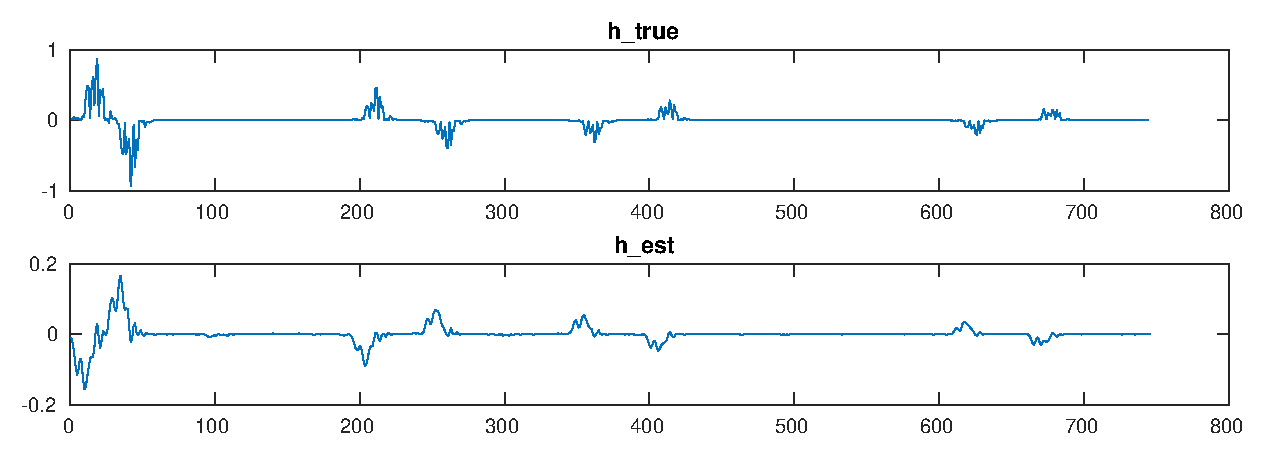
\includegraphics[width=\textwidth]{figures/bce_rec_02_h_trim.pdf}
   \end{center}
\end{frame}

\begin{frame}{Example estimation}
   Still a work in progress!\\
   \begin{center}
      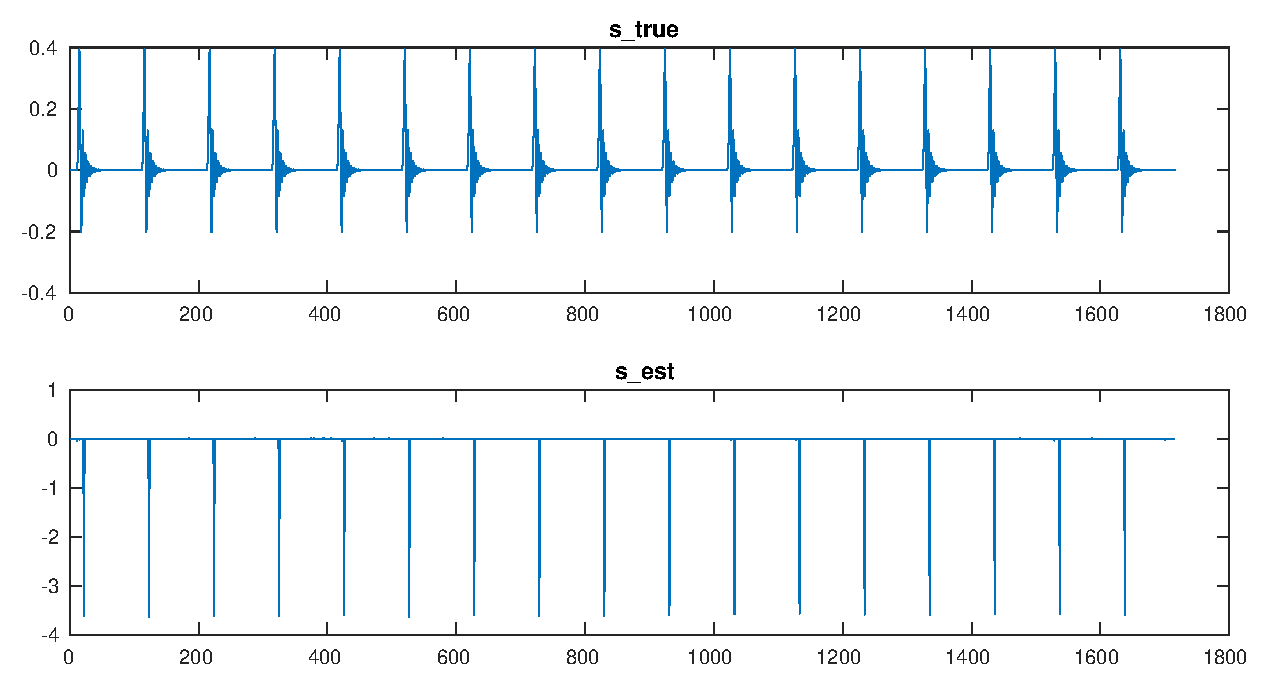
\includegraphics[width=\textwidth]{figures/bce_rec_02_s_trim.pdf}
   \end{center}
\end{frame}


% ]]]

\begin{frame}{Thanks!}
   We can now compute the adjoint wavelet transform:

   \[ \mathcal{W}^\ast = \tilde{\mathcal{W}}_\text{zpd}^\dagger(\mathcal{E}^\dagger)^\ast. \] 
   
   Interesting adjoint in blind channel estimation problem:

   \[ x = h\ast s = \mathcal{A}(hs^T). \] 
   References:
   \begin{itemize}
      \item A. Beck, M. Teboulle, \emph{A Fast Iterative Shrinkage-Thresholding Algorithm for Linear Inverse Problems}, SIAM Journal on Imaging Science, (2009).
      \item A. Ahmed, B. Recht, J. Romberg, \emph{Blind Deconvolution using Convex Programming}, IEEE Trans. on Info. Theory, (2013).
   \end{itemize}
\end{frame}

%XXX Extra slides

% some proximal gradient details
% [[[
\begin{frame}{Proximal Gradient Method}
   \[ f(x) = \dfrac{1}{2}\|\mathcal{A}x-b\|_2^2, \quad g(x) = \lambda \|x\|_1. \] 

   We can use a variant of simple gradient descent to solve the generic problem

   \[ \min_x f(x) + g(x). \] 

   %XXX dropping k step notation for brevity.  x^+ is the new x after the prox grad step
   Proximal gradient method:
   \[ x^{+} = \operatorname{prox}_{t g}\left(x - t\nabla f(x)\right), \text{ step size $t>0$}. \] 
   
   Proximity function: 
   \[ \operatorname{prox}_g(x) \defeq \argmin_u\left(g(u) + \dfrac{1}{2}\|u-x\|_2^2\right). \] 

\end{frame}

\begin{frame}{Proximal Gradient Method}
   %\[ x^{(k)} = \operatorname{prox}_{t_k g}\left(x^{(k-1)} - t_k\nabla f(x^{(k-1)})\right). \] 
   \[ \operatorname{prox}_g(x) \defeq \argmin_u\left(g(u) + \dfrac{1}{2}\|u-x\|_2^2\right). \] 

   For $g(x) = \lambda\|x\|_1$, proximity operator is ``shrinkage'':

   \[ \left\{\operatorname{prox}_g(x)\right\}_i = \left\{\begin{array}{ll} x_i-\lambda & x_i \ge \lambda\\0 & |x_i| < \lambda\\ x_i + \lambda & x_i\le -\lambda\end{array}\right.. \] 

   %XXX dropping k step notation for brevity.  x^+ is the new x after the prox grad step
   Proximal gradient step minimizes $g(u)$ plus quadratic local model of $f(u)$ about $x$:

   \begin{align*}
      x^+ &= \operatorname{prox}_{t g}\left(x - t\nabla f(x)\right)\\
              %&= \argmin_u\left(g(u) + \dfrac{1}{2t}\left\|u-x+t\nabla f(x)\right\|_2^2\right)\\
              &= \argmin_u\left(g(u) + f(x) + \left\langle \nabla f(x), u-x\right\rangle + \dfrac{1}{2t}\|u-x\|_2^2\right).
   \end{align*}

\end{frame}
% ]]]


% proximal gradient and FISTA side-by-side
% [[[
\begin{frame}{Proximal Gradient and FISTA}
   Proximal gradient:\\
   \begin{itemize}
      \item Choose $x^{(0)}$.
      \item For $k=1,2,...$\\[-1em]

         \[ x^{(k)} = \operatorname{prox}_{t_k g}\left(x^{(k-1)} - t_k\nabla f(x^{(k-1)})\right), \text{ with step size $t_k$.} \] 
   \end{itemize} 

   FISTA (fast iterative shrinkage-thresholding algorithm):\\
   \begin{itemize}
      \item Choose $x^{(0)}=x^{(-1)}$.
      \item For $k=1,2,...$\\[-1em]
         \[ y = x^{(k-1)} + \dfrac{k-2}{k+1}\left(x^{(k-1)}-x^{(k-2)}\right) \] 
         \[ x^{(k)} = \operatorname{prox}_{t_kg}\left(y - t_k\nabla f(y)\right), \text{ with step size $t_k$.} \] 
   \end{itemize}

\end{frame}
% ]]]


% analysis formulation
% [[[
\begin{frame}{Analysis formulation}
   \begin{columns}
      \begin{column}{0.5\textwidth}
         Synthesis formulation\\[-1em]
         \[ \min_x \dfrac{1}{2}\|\mathcal{RW}x-b\|_2^2 + \lambda \|x\|_1 \]

         $x$ contains coefficients.\\
      \end{column}

      \begin{column}{0.5\textwidth}
         Analysis formulation\\[-1em]
         \[ \min_y \dfrac{1}{2}\|\mathcal{R}y-b\|_2^2 + \lambda \|\mathcal{W}^\dagger y\|_1 \] 

         $y$ is an image.
      \end{column}
   \end{columns}
   
   ~\\
   In the analysis formulation, we need $\operatorname{prox}_g(y)$ with $g(y) = \lambda\|\mathcal{W}^\dagger y\|_1$ instead of just $\lambda\|x\|_1$.\\[1em]

   We know how to compute the prox function if $\mathcal{W}^\dagger(\mathcal{W}^\dagger)^\ast = \nu I$.  This is okay for orthogonal wavelets, but not for biorthogonal wavelets.  But it's ``close'' in practice.\\[1em]
   
   P. Combettes, J.-C. Pesquet, \emph{A Douglas-Rachford splitting approach to nonsmooth convex variational signal recovery}, IEEE Journal of Selected Topics in Signal Processing, (2007).
\end{frame}
% ]]]


% original cameraman and recovered images side-by-side
% [[[
\begin{frame}{Image Deblurring Problem}
   $200$ iterations of FISTA, $\mathcal{W}^\dagger$ is a 3-stage CDF 9/7 wavelet transform, ${\lambda = 2\times 10^{-5}}$
   \begin{center}
   \begin{columns}[t]
      \begin{column}{0.45\textwidth}
         Original image:
         \includegraphics[width=\textwidth]{../ieee_spm/figures/{cameraman}.pdf}

      \end{column}
      
      \begin{column}{0.45\textwidth}
         Using $\mathcal{W}^\ast = \tilde{\mathcal{W}}_\text{zpd}^\dagger(\mathcal{E}^\dagger)^\ast$:
         \includegraphics[width=\textwidth]{../ieee_spm/figures/{cameraman_rec_200_bior4.4_sym_trim}.pdf}
         \[ \scalemath{0.75}{\dfrac{\|\mathcal{W}x-y\|_2}{\|y\|_2} = 7.24\times 10^{-2}} \] 
      \end{column}
   \end{columns}
   \end{center}

\end{frame}

% ]]]


% some extra BCE recoveries (more-or-less cherry picked!)
% [[[
\begin{frame}{Example estimation}
   Still a work in progress!\\
   \begin{center}
      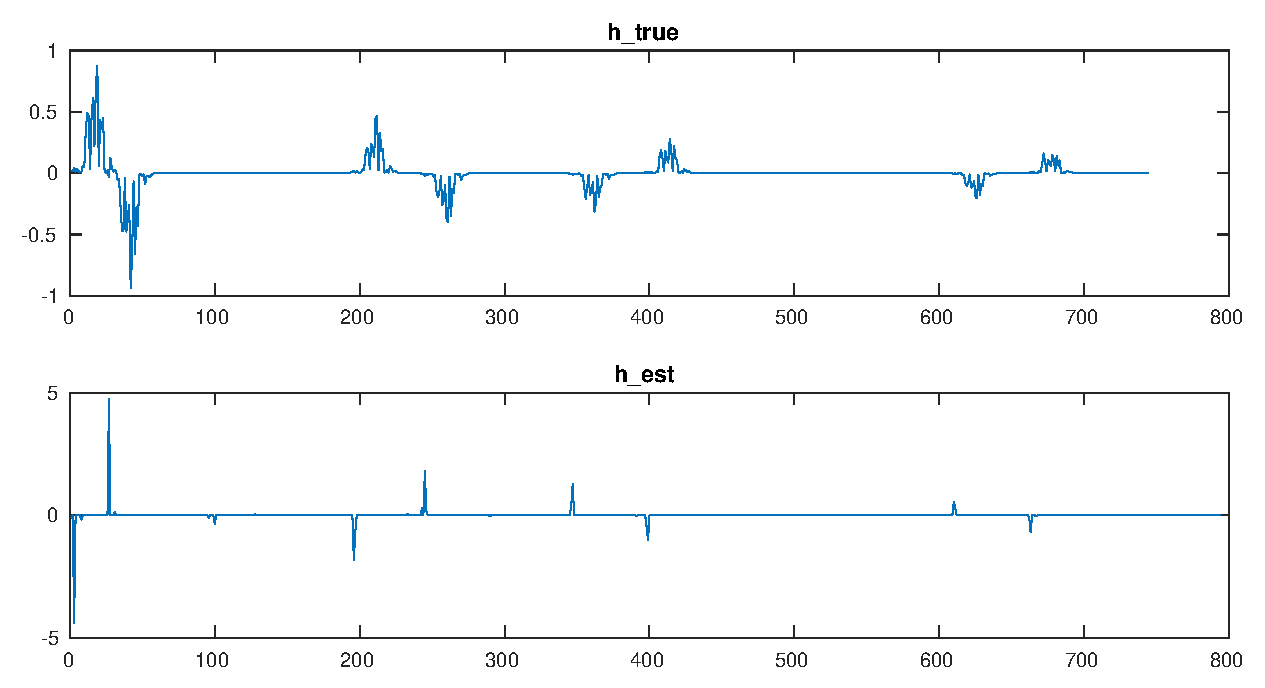
\includegraphics[width=\textwidth]{figures/bce_rec_03_h_trim.pdf}
   \end{center}
\end{frame}

\begin{frame}{Example estimation}
   Still a work in progress!\\
   \begin{center}
      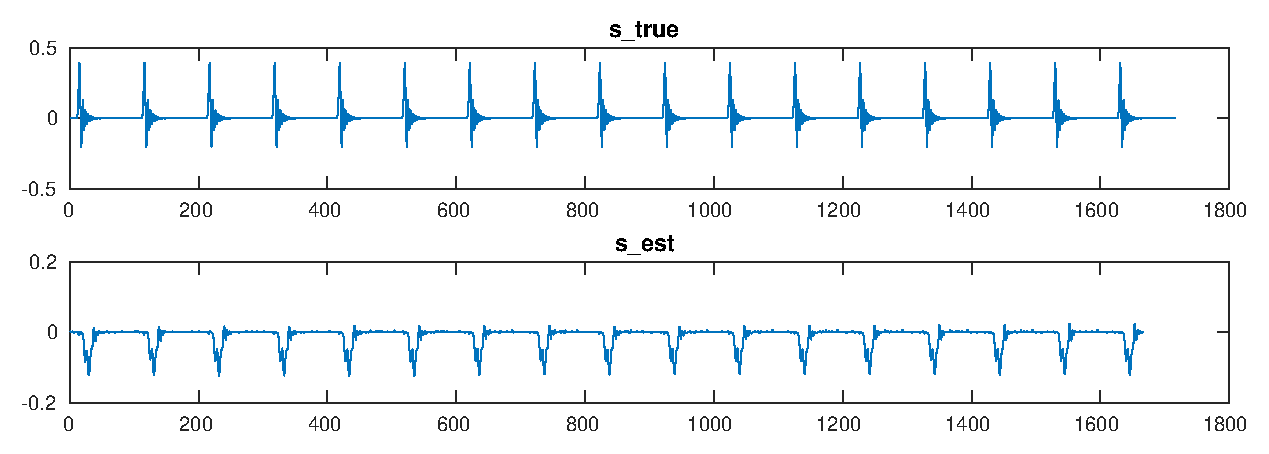
\includegraphics[width=\textwidth]{figures/bce_rec_03_s_trim.pdf}
   \end{center}
\end{frame}
% ]]]


\end{document}

% vim: set spell:
% vim: foldmarker=[[[,]]]

